\section{H67: The talk loop sits far below runaway}
\label{sec:H67}

\textbf{The question:} When one agent posts a message, how many extra messages does it cause through other agents reading it? Is this loop gain close to 1, where talk cascades run away? Does a dial on the read-out call see more gain than the one-minute equal-time dial of H25?

\textbf{The intuition:} Think of a microphone near a speaker. Each sound comes back multiplied by the loop gain $g$. If $g<1$, a push dies out, and the total amplification is $\chi=1/(1-g)$. At $g=1$ the system howls; this is the critical point. In a branching process, $g$ is the mean number of offspring of one event. Here the offspring are talk messages that reading causes. The scaffold lets an agent read new messages only at its next model call, the read-out call. So the response should appear at that call. The equal-time dial counts co-movement inside one minute. It can therefore mistake a shared field (all agents reacting to the same burst or schedule) for coupling.

\begin{figure}[h]
\includegraphics[width=\textwidth]{H67-subcritical-dial/fig.pdf}
\caption{The talk loop sits far below its critical point. (a) The amplification $\chi=1/(1-g)$ against the loop gain, with every goal period at its read-out gain; no period passes 0.23, against a divergence at 1. (b) The read-out gain per period in time order: about 0 in regimes I and II and about 0.13 in regime III, with the equal-time dial (orange) reading higher from shared fields. Animation: \texttt{writeup/animations/H67-subcritical-dial.mp4}.}
\label{fig:int-H67}
\end{figure}
\begin{figure}[h]
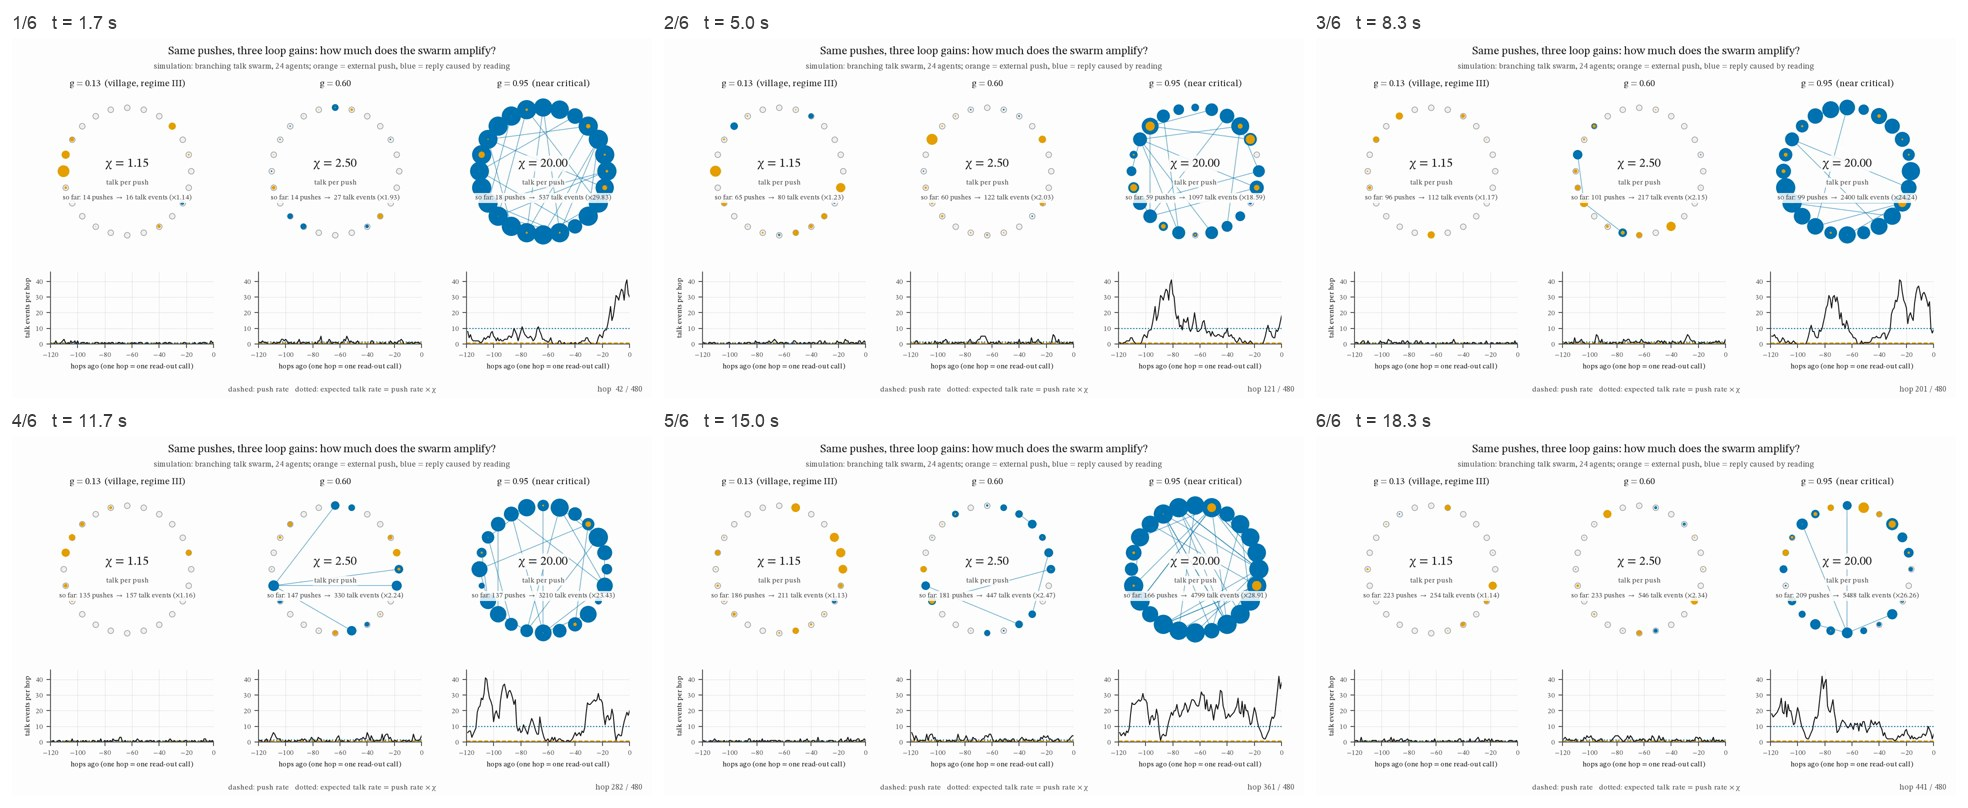
\includegraphics[width=0.9\textwidth]{storyboards/H67.jpg}
\caption{Animation storyboard: six frames of the animation, evenly spaced in time (frame number and time above each). The full animation is \texttt{writeup/animations/H67-subcritical-dial.mp4}.}
\end{figure}


\textbf{What we measured:} The read-out jump $J_1^*$ is the extra talk probability per peer message read at a call. We subtract the effect of messages posted while the call was running (the in-flight placebo, at matched lag). Those messages share every local field, but the call cannot read them. The loop gain is $g_\mathrm{lag}=\bar m\,\bar r\,J_1^*$: messages per talk call times readers per message times the jump. We fit it within each of 66 units in 35 goal periods, on 1.47M receiving calls inside all-present windows.
Impostors: all four are removed. \emph{Scheduler field:} each call is one update with agent $\times$ day $\times$ call-class baselines. The placebo cancels any field that is smooth over one call latency (5--60\,s). \emph{External drive:} human messages and nudges are covariates, and the placebo shares any kickoff burst. \emph{Shared model prior:} agent $\times$ day baselines absorb each agent's talk rate, so only timing identifies the coupling. \emph{Common input:} the in-flight placebo is exactly the ``posted but not yet read'' control.
The synthetic check ran on the real call grids. Planted gains of 0.15--0.60 came back with bias $-1\%$ to $-3\%$ and interval coverage 0.88--0.98. A world with fields only gave $-0.010$. A burst world gave $-0.03$, where the uncorrected gain reads $+0.06$.

\textbf{What we found:} The read-out loop gain of talk is subcritical in 66/66 units\cred{0.79}; EU 2.17 (value if true 2.75). Every unit's upper bound is below 0.40. The regime-III median is 0.13, and \#51 gives $0.142$ $[0.111, 0.174]$. Regime I gives 0.005. The largest goal-period gain is 0.234, so $\chi\le1.31$. At the median, $\chi\approx1.15$ and $T/T_c\approx8$: the swarm runs eight times hotter than its critical point. The coupling acts mostly on named messages. A named message raises the recipient's talk probability by $0.079$ $[0.069, 0.089]$ per read; an unnamed one by $0.004$ $[0.003, 0.006]$ ($\times19$). Named messages give about half of the gain. In \#51 the gain stays flat (0.14) as the swarm grows from 21 to 32 agents. The per-read jump falls with headcount ($\rho=-0.59$). The gain ranks periods like H42's read-out Hawkes fit ($\rho=0.55$, $p=0.0007$). The original claim (lagged gain $>$ equal-time dial) fails: it holds in only 7/35 periods. The equal-time dial reads 0.10--0.31 from fields alone.
The scope is 66 units in 35 goal periods, with the native tests NE14, NE42 and G51.

\textbf{What it means:} For a monitor, report $g_\mathrm{lag}$, not the equal-time dial, as the distance to runaway talk. Expect a push to grow by at most $\times1.31$. No village configuration from 4 to 32 agents came near runaway, so this is a gauge, not a lever. For an operator who wants a reply, name the recipient: that raises its next-call talk probability by 0.08 instead of 0.004. For a scaffold builder, more agents do not push the swarm toward criticality, because each read counts for less.

\textbf{Caveats:} Only the first hop has a placebo correction. Hops 2--3 (median 0.28) have none. Regime-I talk happens at scheduled chat calls, so this estimator uses the wrong clock there. A post hoc subset of quiet recipients lowers the regime-III median to 0.086 ($-34\%$). The unnamed part sits at the resolution of the placebo (bias about $\pm0.03$ in $g$). The shift null rejects in 13.6\% of units (synthetic 7.5--10\%), so single-unit significance is slightly optimistic. H50's estimator gives about twice this gain ($\rho=0.24$). The predictions were written with H25, H42 and H50 known. No confirmation test on reserved goal periods has run.
